\documentclass[aspectratio=169,11pt]{beamer}
\usepackage{amsmath,amssymb,booktabs,tikz,listings}
\usetikzlibrary{arrows.meta,positioning,calc}
\definecolor{blue}{HTML}{285BC2}
\definecolor{water}{HTML}{258BD2}
\definecolor{ink}{HTML}{25282D}
\definecolor{muted}{HTML}{646E7B}
\definecolor{red}{HTML}{BA463A}
\setbeamercolor{normal text}{fg=ink,bg=white}
\setbeamercolor{structure}{fg=blue}
\setbeamercolor{frametitle}{fg=blue}
\setbeamercolor{itemize item}{fg=blue}
\setbeamerfont{frametitle}{size=\Large,series=\bfseries}
\setbeamerfont{title}{size=\Huge,series=\bfseries}
\setbeamertemplate{navigation symbols}{}
\setbeamertemplate{itemize item}{\small$\bullet$}
\setbeamertemplate{footline}{\hfill\color{muted}\scriptsize\insertframenumber\,/\,\inserttotalframenumber\hspace{7mm}\vspace{4mm}}
\setbeamersize{text margin left=9mm,text margin right=9mm}
\lstset{basicstyle=\ttfamily\footnotesize,columns=fullflexible,
  keepspaces=true,showstringspaces=false,keywordstyle=\color{blue},
  morekeywords={if,return,for,in,while,push,pop,then,else},aboveskip=5pt}
\newcommand{\src}[1]{\vfill{\tiny\color{muted}#1}}
\newcommand{\pipearm}[3]{\draw[draw=#3,line width=3pt,line cap=round] (#1,#2) -- ++(0.43,0);}
% A tile's integer mask uses N=1, E=2, S=4, W=8.
\newcommand{\tile}[4]{%
  \begin{scope}[shift={(#1,#2)}]
    \draw[gray!25] (-.5,-.5) rectangle (.5,.5);
    \foreach \bit/\dx/\dy in {1/0/0.5,2/0.5/0,4/0/-0.5,8/-0.5/0}{%
      \pgfmathtruncatemacro{\hasport}{mod(floor(#3/\bit),2)}
      \ifnum\hasport=1
        \draw[#4,line width=3.6pt,line cap=round] (0,0)--(\dx,\dy);
      \fi}
  \end{scope}}
\newcommand{\board}[2]{%
  \foreach \mask [count=\idx from 0] in {#1}{%
    \pgfmathtruncatemacro{\col}{mod(\idx,4)}
    \pgfmathtruncatemacro{\row}{-floor(\idx/4)}
    \tile{\col}{\row}{\mask}{#2}}
  \fill[white] (2,-2) circle (.15);
  \fill[blue] (2,-2) circle (.11);}

\begin{document}

% 1
\begin{frame}[plain]
\begin{columns}[c,onlytextwidth]
\column{.60\textwidth}
{\color{blue}\Huge\bfseries Pipes}\par\vspace{4mm}
{\Large Search for a connected network}\par\vspace{7mm}
Introduction to Artificial Intelligence\par\vspace{3mm}
\small Depth-first search and Greedy Best-First\par
\column{.34\textwidth}
\centering
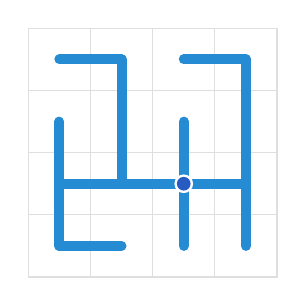
\begin{tikzpicture}[scale=.79]
\board{2,12,2,12,4,5,4,5,7,11,15,13,3,8,1,1}{water}
\end{tikzpicture}
\end{columns}
\end{frame}

% 2
\begin{frame}{Goal: one connected, acyclic network}
\begin{columns}[c,onlytextwidth]
\column{.38\textwidth}\centering
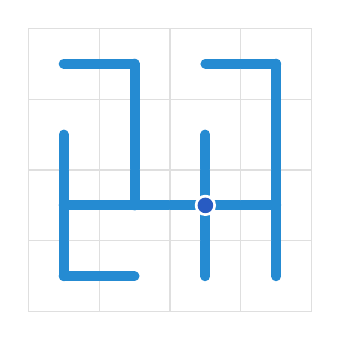
\begin{tikzpicture}[scale=.9]
\board{2,12,2,12,4,5,4,5,7,11,15,13,3,8,1,1}{water}
\end{tikzpicture}
\column{.57\textwidth}
\begin{itemize}
\item Every port matches its neighbor.
\item No port leaves the grid.
\item All tiles connect. No cycles.
\end{itemize}
\vspace{4mm}
Tiles are vertices, connections are edges.
\[
G\text{ is a tree} \quad\Longrightarrow\quad |E|=n-1
\]
\small The blue source anchors water visualization.
\end{columns}
\src{Rules: puzzle-pipes.com. Goal validation: model.py and search.py.}
\end{frame}

% 3
\begin{frame}{Problem formulation}
\small
\begin{tabular}{@{}p{.23\textwidth}p{.70\textwidth}@{}}
\toprule
Input & $n=m^2$ tiles, fixed shapes, ordinary boundaries \\
State & Prefix $s=(a_0,\ldots,a_{k-1})$ of assigned orientations \\
Initial state & Empty prefix $()$, with all tile shapes known \\
Action & Assign a rotation to tile $k$ in row-major order \\
Transition & $s'=s+(a_k)$, accepted after feasibility checks \\
Goal & $k=n$ and the complete board passes all rules \\
Cost & Unit assignment cost, unused by either ranking \\
\bottomrule
\end{tabular}\par
\vspace{5mm}
\normalsize A solver assignment can represent several manual clicks.\par
\small Any valid solution is acceptable. Minimum-click solutions are outside scope.
\src{Implemented state model: Search in pipes\_problem/search.py.}
\end{frame}

% 4
\begin{frame}{Legal successors}
The next tile has a fixed shape. Search chooses its orientation.
\vspace{5mm}
\begin{center}
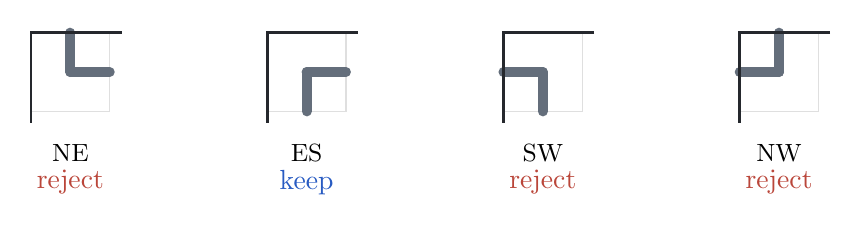
\begin{tikzpicture}[x=1cm,y=1cm]
\foreach \mask/\x/\label in {3/0/NE,6/3/ES,12/6/SW,9/9/NW}{
  \begin{scope}[shift={(\x,0)}]
    \tile{0}{0}{\mask}{muted}
    \draw[ink,line width=1pt] (.65,.5)--(-.5,.5)--(-.5,-.65);
    \node[below=8mm] at (0,0) {\small\label};
  \end{scope}}
\node[red] at (0,-1.4) {reject};
\node[blue] at (3,-1.4) {keep};
\node[red] at (6,-1.4) {reject};
\node[red] at (9,-1.4) {reject};
\end{tikzpicture}
\end{center}
\small Top-left corner example. The left and top borders forbid N and W.\par
\vspace{4mm}
\normalsize Neighbor matching also checks absent ports.\par
\small A candidate must pass every shared pruning check before search accepts it.
\src{Example is schematic. Orientation filtering: boundary\_domains() and compatible().}
\end{frame}

% 5
\begin{frame}{Search space}
\begin{columns}[T,onlytextwidth]
\column{.48\textwidth}
\small Distinct rotations per tile\par\vspace{3mm}
\begin{tabular}{@{}lr@{}}\toprule
End, elbow, T-junction & 4\\
Straight & 2\\
Cross & 1\\\bottomrule
\end{tabular}
\vspace{4mm}
\normalsize
\[U=\prod_{i=0}^{n-1}|R_i|\leq 4^n\]
\small Complete assignments before boundary checks.
\column{.47\textwidth}
\small Prefix tree\par\vspace{3mm}
\begin{tikzpicture}[every node/.style={font=\small},level distance=10mm,
 level 1/.style={sibling distance=24mm},level 2/.style={sibling distance=11mm}]
\node {$()$}
 child {node {$a_0$} child {node {$a_1$}} child {node {$a'_1$}}}
 child {node {$a'_0$} child {node {$\cdots$}}};
\end{tikzpicture}
\par\small Depth $n$, branching factor at most 4.\par
Each prefix has one parent.
\end{columns}
\vspace{4mm}
For the shipped 4\,$\times$\,4 example: $U=268{,}435{,}456$.\par
\small This bound counts assignments, not measured expansions.
\src{Count derived from distinct rotations in pipes-4x4-261.json.}
\end{frame}

% 6
\begin{frame}{Shared pruning}
\centering
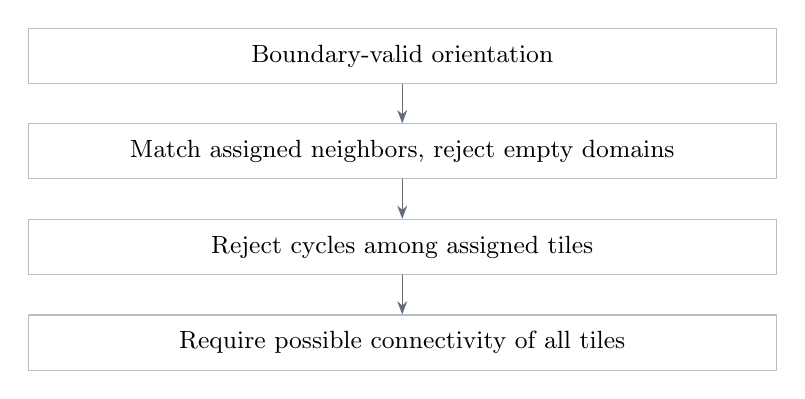
\begin{tikzpicture}[node distance=5mm,
 test/.style={draw=muted!45,minimum width=95mm,minimum height=7mm,font=\small},
 link/.style={-{Stealth},draw=muted}]
\node[test] (a) {Boundary-valid orientation};
\node[test,below=of a] (b) {Match assigned neighbors, reject empty domains};
\node[test,below=of b] (c) {Reject cycles among assigned tiles};
\node[test,below=of c] (d) {Require possible connectivity of all tiles};
\draw[link] (a)--(b);\draw[link] (b)--(c);\draw[link] (c)--(d);
\end{tikzpicture}
\vspace{3mm}\par
\small Both solvers use identical checks and fixed tile order.\par
\vspace{2mm}
Root condition: total ports $=2(n-1)$.\par
Possible connectivity is necessary but does not prove a solution exists.
\src{Pruning implementation: Search.compatible(). Full reasoning: docs/pipes-analysis.md.}
\end{frame}

% 7
\begin{frame}[fragile]{Depth-first search}
\begin{columns}[T,onlytextwidth]
\column{.60\textwidth}
\begin{lstlisting}
VISIT(s):
  if budget exhausted: return LIMIT
  count expansion
  if GOAL(s): return SOLVED(s)
  for a in rotations of tile |s|:
    child = s + (a)
    if FEASIBLE(child):
      r = VISIT(child)
      if r is SOLVED or LIMIT: return r
  return UNSOLVABLE
\end{lstlisting}
\column{.35\textwidth}
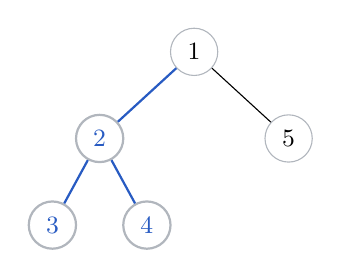
\begin{tikzpicture}[level distance=11mm,
 level 1/.style={sibling distance=24mm},level 2/.style={sibling distance=12mm},
 every node/.style={circle,draw=muted!50,minimum size=6mm,font=\small}]
\node {1}
 child[blue,thick] {node {2} child {node {3}} child {node {4}}}
 child {node {5}};
\end{tikzpicture}
\par\vspace{3mm}\small Schematic visit order.\par
Explore a branch, then backtrack.
\end{columns}
\vspace{4mm}
\small Finite-tree completeness with sufficient resources and sound pruning.\par
Worst-case exploration remains exponential.
\src{Simplified pseudocode matches dfs(). Root feasibility precedes VISIT. Cancellation is external.}
\end{frame}

% 8
\begin{frame}{Greedy's heuristic: remaining choices}
\[
h(s)=\sum_{i\text{ unassigned}}\log_2 |D_i(s)|
\]
\small $D_i(s)$ contains boundary-valid orientations matching assigned neighbors.
\vspace{5mm}
\begin{center}
\begin{tabular}{@{}lcc@{}}
\toprule
Candidate & Remaining domain sizes & $h(s)$\\\midrule
A & $(1,2,4)$ & $0+1+2=3$\\
B & $(1,1,2)$ & $0+0+1=1$\\\bottomrule
\end{tabular}
\end{center}
\vspace{3mm}
Greedy prefers B. Smaller values indicate fewer unresolved choices.\par
\small Tie order: deeper prefix, then earlier insertion.\par\vspace{3mm}
The score ignores dependencies between unassigned tiles.\par
It provides no admissibility or minimum-click guarantee.
\src{Hypothetical domain example. Exact priority: (h, -depth, insertion order) in greedy().}
\end{frame}

% 9
\begin{frame}[fragile]{Greedy Best-First search}
\begin{columns}[T,onlytextwidth]
\column{.61\textwidth}
\begin{lstlisting}
push () into min-priority queue
while queue is not empty:
  if budget exhausted: return LIMIT
  s = pop minimum-priority state
  count expansion
  if GOAL(s): return SOLVED(s)
  for a in rotations of tile |s|:
    child = s + (a)
    D = FEASIBLE(child)
    if D exists:
      push child with (h(child),
                       -|child|, serial)
return UNSOLVABLE
\end{lstlisting}
\column{.34\textwidth}
\small Queue selection\par\vspace{3mm}
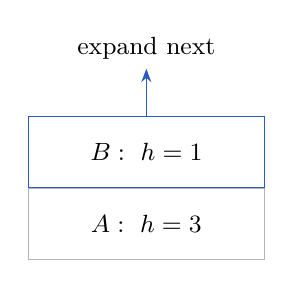
\begin{tikzpicture}[every node/.style={font=\small}]
\node[draw=blue,minimum width=30mm,minimum height=9mm] (b) {$B:\ h=1$};
\node[below=0mm of b,draw=muted!50,minimum width=30mm,minimum height=9mm] (a) {$A:\ h=3$};
\node[above=6mm of b] (pop) {expand next};
\draw[-{Stealth},blue] (b)--(pop);
\end{tikzpicture}
\par\vspace{3mm}
All feasible prefixes remain queued.\par\vspace{3mm}
Memory can grow exponentially.
\end{columns}
\src{Root feasibility precedes the queue. Priority uses h alone. The unique root starts at zero.}
\end{frame}

% 10
\begin{frame}{Evaluation protocol}
\begin{itemize}
\item Same nine saved maps for both algorithms.
\item Three maps per size, five repeats per algorithm.
\item Shared pruning, tile order and resource limits.
\end{itemize}
\vspace{4mm}
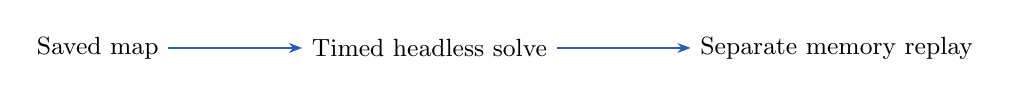
\begin{tikzpicture}[every node/.style={font=\small},node distance=17mm]
\node (map) {Saved map};
\node[right=of map] (time) {Timed headless solve};
\node[right=of time] (mem) {Separate memory replay};
\draw[-{Stealth},blue] (map)--(time);
\draw[-{Stealth},blue] (time)--(mem);
\end{tikzpicture}
\vspace{4mm}\par
\small Time excludes drawing and playback. Peak memory counts traced Python
allocations. Combine passes only when outcomes agree.\par\vspace{3mm}
Limits: 30 seconds of solver computation and 200,000 expansions.
\src{Runner: benchmark.py. Measurement: measure() and worker.py.}
\end{frame}

% 11
\begin{frame}{Baseline results}
% Source: docs/benchmarks/2026-10-22.csv, successful-run group medians.
\begin{center}
\small
\begin{tabular}{@{}llrrr@{}}
\toprule
Size & Algorithm & Solved/runs & Time (ms) & Peak (KiB)\\
\midrule
$4\times4$ & DFS    & 15/15 & 0.685 & 26.984\\
           & Greedy & 15/15 & 0.776 & 12.359\\
$5\times5$ & DFS    & 15/15 & 1.518 & 53.297\\
           & Greedy & 15/15 & 1.692 & 19.219\\
$7\times7$ & DFS    & 15/15 & 6.603 & 145.852\\
           & Greedy & 15/15 & 8.213 & 27.594\\
\bottomrule
\end{tabular}
\end{center}

\vspace{3mm}
\small Median over 15 successful runs per size and algorithm.\par
Each group contains three distinct inputs with five timing repeats.\par\vspace{3mm}
These inputs require little search under shared pruning. Queue overhead can outweigh
the benefit of Greedy's ranking. This small sample supports no general winner.
\src{Measured 22 October 2026. Raw rows and environment: docs/benchmarks/.}
\end{frame}

% 12
\begin{frame}{Scope and next experiments}
\begin{itemize}
\item Compare harder maps and proven-unsolvable inputs.
\item Measure the effect of shared pruning separately.
\item Keep UNSOLVABLE distinct from LIMIT or CANCELLED.
\item Complete the second puzzle and final course report.
\end{itemize}
\vspace{5mm}
\small\textbf{References}\par\vspace{2mm}
Pipes rules: \url{https://www.puzzle-pipes.com/}\par
Russell and Norvig, \emph{Artificial Intelligence: A Modern Approach},
4th ed., Chapters 3 and 6. \url{https://aima.cs.berkeley.edu/}\par\vspace{2mm}
Implementation and derived analysis: this repository's
\texttt{search.py}, \texttt{model.py} and \texttt{docs/pipes-analysis.md}.
\end{frame}

\end{document}
